\section{Local Optimization}

After having implemented the four above heuristics, we tried to implement some local optimization methods. These methods take a given tour and try to enhance it. Three main techniques are commonly used : 2-opt, 3-opt and Lin-Kernighan.

\subsection{2-opt}
 The idea of 2-opt is to try to exchange all the pairs of edges (see example in Figure~\ref{2-opt}). In the implementation of this method, we have to be careful to the direct
 \begin{figure}[!h]
	\begin{center}
		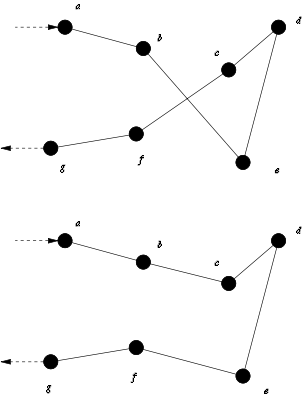
\includegraphics[width=5cm]{images/2opt.png}
		\caption{Example of permutation}
		\label{2-opt}
	\end{center}
\end{figure}

 \subsection{3-opt}
 
 